%vim: tw=8 gqap formata paragrafos gq formata selecao
\documentclass[12pt]{article}
\usepackage{sbc-template}
\usepackage{graphicx,url}
\usepackage[brazil]{babel}
\usepackage[utf8]{inputenc}
\usepackage{multicol}

\sloppy

\title{Redes de Software Sintéticas Aplicadas à Avaliação de Algoritmos de
Recuperação de Modularização}

\author{Rodrigo Rocha Gomes e Souza\inst{1}
%, Dalton Guerrero\inst{1}, Jorge Figueiredo\inst{1}
}

\address{Departamento de Sistemas e Computação\\
Universidade Federal de Campina Grande (UFCG)\\ 
Caixa Postal 10.106 -- CEP 58.109-970 \\
Campina Grande -- PB -- Brazil
\email{rodrigo@dsc.ufcg.edu.br} }

\begin{document} 

\maketitle

\begin{abstract} 

Software modularization recovery algorithms automatically recognize a system's
modular structure by analyzing its implementation. Because the empirical
evaluation of these algorithms depends on the availability test sets composed by
systems with documented modular structure, most empirical studies are, in fact,
small case studies that cannot be generalized. We propose an evaluation method
which uses software models capable of producing arbitrary-sized test sets. We
hope this approach will increase the available knowledge about the algorithms
and how they can be improved.
% TODO Abstracts should not have more than 10 lines and must be in the first
% page of the paper.

\end{abstract}
     
\begin{resumo} 

% XXX não é A estrutura de módulos, é UMA
Algoritmos de recuperação modularização de \emph{software} procuram identificar
automaticamente a estrutura de módulos de um sistema de \emph{software} a partir
de sua implementação. Como a avaliação empírica desses algoritmos depende da
disponibilidade de um conjunto de testes formado por sistemas cuja organização
modular é bem documentada, a maioria dos estudos empíricos são pequenos estudos
de caso que não podem ser generalizados.  Propomos uma forma de avaliação que
usa modelos de \emph{software} para produzir conjuntos de teste de tamanho
arbitrário.  Esperamos com isso aumentar o conhecimento disponível sobre os
algoritmos e sobre como eles podem ser melhorados.
% O resumo (e o abstract) não ultrapassem 10 linhas cada, sendo que ambos devem
% estar na primeira página do artigo.

\end{resumo}

%%%%%%%%%%%%%%%%%%%%%%%%%%%%%%%%%%%%%%%%%%%%%%%%%%%%%%%%%%%%%%%%%%%%%%%%%%%%%%
%%%%%%%%%%%%%%%%%%%%%%%%%%%%%%%%%%%%%%%%%%%%%%%%%%%%%%%%%%%%%%%%%%%%%%%%%%%%%%
\section{Introdução}
% "Introdução" caracterizando o contexto em que o trabalho se insere;

A divisão conceitual de um sistema de \emph{software} em módulos é uma
informação valiosa durante o seu desenvolvimento. Uma boa organização modular
revela subconjuntos de um sistema que podem ser desenvolvidos por equipes
trabalhando de forma mais ou menos independente, o que contribui para reduzir o
tempo de implementação. Apesar disso, o conhecimento sobre a organização de um
sistema muitas vezes é mal documentado e acaba se perdendo à medida que os
desenvolvedores são substituídos \cite{Clements2002}. % cit Parnas?

Algoritmos de recuperação de modularização de \emph{software} procuram extrair
da implementação de um sistema uma organização modular e, por isso, auxiliam a
divisão de tarefas entre desenvolvedores.  Para realizar a decomposição de um
sistema em módulos, muitos desses algoritmos usam heurísticas baseadas nas
dependências existentes entre os componentes básicos da implementação do
sistema.

Em sistemas implementados em linguagens orientadas a objetos, os componentes
básicos são as classes e as interfaces, as quais se relacionam através de
mecanismos como herança e agregação. Essas relações estabelecem dependências
entre os componentes que, unidas, formam uma rede de dependências, também
chamada de rede de \emph{software}. Formalmente, a entrada de um algoritmo de
recuperação de modularização é uma rede de \emph{software}, modelada como
grafo orientado, e a saída é uma rede modular resultante do particionamento em
módulos da rede original, como mostra a Figura \ref{fig:rede-modular}. Os
vértices do grafo representam componentes e as arestas, relações de dependência
entre componentes.


Recentemente alguns pesquisadores analisaram redes de \emph{software} sob a luz
da teoria das redes complexas e encontraram propriedades topológicas marcantes
que também estão presentes em redes de interações entre proteínas, redes
sociais e muitas outras \cite{Myers2003,Valverde2003}. Descobriu-se que nessas
redes a distribuição dos graus dos vértices é bem aproximada por uma lei de
potência, $N(k) \sim k^{-\gamma}$, ou seja, o número de vértices ligados a
exatamente $k$ arestas é proporcional a uma potência de $k$ com expoente
negativo e constante, como mostra a Figura \ref{fig:leidepotencia}. Redes
caracterizadas por essa distribuição de graus específica são chamadas de redes
livres de escala. % \cite{Barabasi1999}.


%\begin{figure}[ht]
%\begin{minipage}[b]{0.5\linewidth}
%\centering
%\includegraphics[scale=1]{filename1}
%\caption{default}
%\label{fig:figure1}
%\end{minipage}
%\hspace{0.5cm}
%\begin{minipage}[b]{0.5\linewidth}
%\centering
%\includegraphics[scale=1]{filename2}
%\caption{default}
%\label{fig:figure2}
%\end{minipage}
%\end{figure}



\begin{figure}[ht]
\begin{minipage}[b]{0.5\linewidth}
\centering
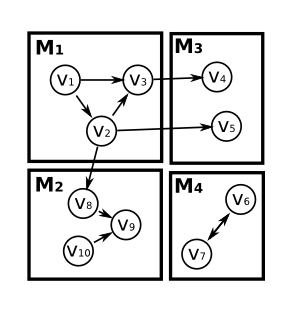
\includegraphics[width=0.6\textwidth]{rede-modular} 
\caption{Uma rede modular com 10 vértices organizados em 4 módulos.} 
\label{fig:rede-modular}
\end{minipage}
\hspace{0.5cm}
\begin{minipage}[b]{0.5\linewidth}
\centering
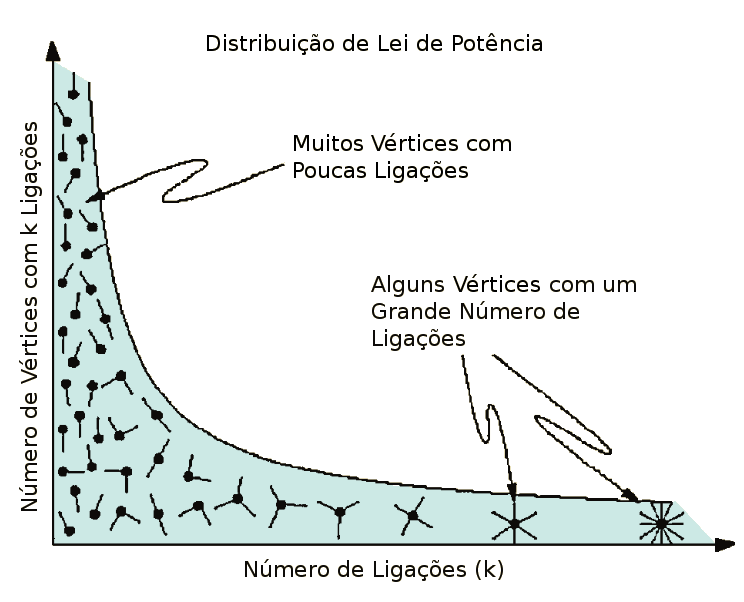
\includegraphics[width=0.9\textwidth]{leidepotencia}
\caption{Distribuição de graus como lei de potência. Adaptado de 
\cite{Barabasi2007}.} 
\label{fig:leidepotencia}
\end{minipage}
\end{figure}

%\begin{figure}
%\centering
%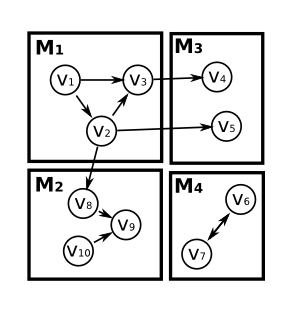
\includegraphics[width=0.3\textwidth]{rede-modular} 
%\caption{Uma rede modular com 10 vértices organizados em 4 módulos.} 
%\label{fig:rede-modular}
%\end{figure}
%
%\begin{figure} 
%\centering
%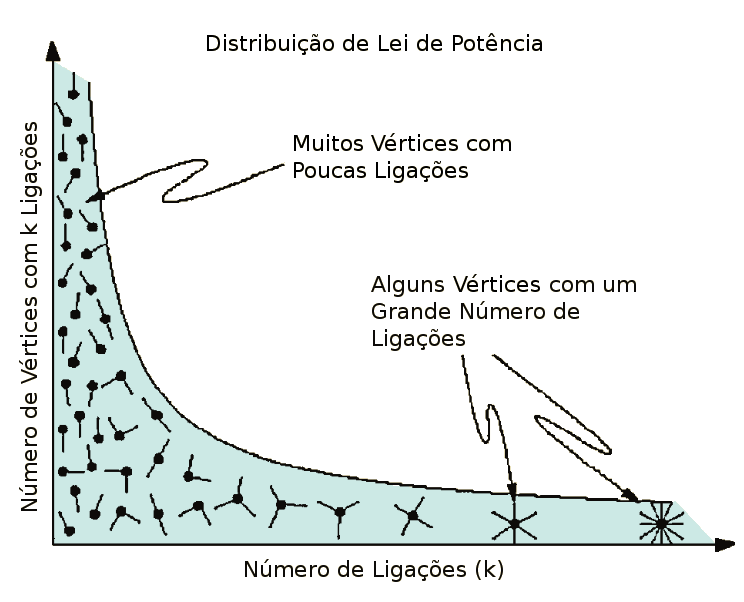
\includegraphics[width=0.5\textwidth]{leidepotencia}
%\caption{Distribuição de graus como lei de potência. Adaptado de 
%\cite{Barabasi2007}.} 
%\label{fig:leidepotencia}
%\end{figure}

Para tentar explicar os mecanismos responsáveis pela formação de redes livres de
escala em diversos domínios, pesquisadores criaram vários modelos estocásticos.
Esses modelos são algoritmos que geram vértices e arestas de maneira
probabilística porém de acordo com certas regras que garantem que, quando o
número de vértices tende a infinito, a distribuição dos graus dos vértices tende
a uma lei de potência. Por essa razão tais modelos podem produzir redes
similares a redes de \emph{software}, ao menos quanto à distribuição de graus.

%%%%%%%%%%%%%%%%%%%%%%%%%%%%%%%%%%%%%%%%%%%%%%%%%%%%%%%%%%%%%%%%%%%%%%%%%%%%%%
%%%%%%%%%%%%%%%%%%%%%%%%%%%%%%%%%%%%%%%%%%%%%%%%%%%%%%%%%%%%%%%%%%%%%%%%%%%%%%
\section{Identificação do Problema} 
% "Identificação do Problema" a ser investigado na pesquisa bem como sua
% relevância para a área de conhecimento;

% MODULARIZAÇÃO DE REFERÊNCIA

Idealmente os algoritmos de recuperação de modularização de \emph{software}
devem encontrar organizações modulares semelhantes àquelas que seriam
encontradas por especialistas nos sistemas analisados. Uma forma de testar os
algoritmos consiste, pois, em aplicá-los à rede de um sistema para o qual
exista uma organização modular de referência e então comparar essa organização
à organização encontrada pelo algoritmo. A diferença entre as organizações
modulares pode ser quantificada por uma métrica de distância entre
particionamentos \cite{Tzerpos1999}.

Infelizmente é difícil encontrar sistemas cuja organização modular é
documentada. Organizações modulares de referência podem ser obtidas através de
um experimento controlado no qual um grupo de programadores experientes analisa
o código-fonte de um sistema e propõe uma organização modular para ele
\cite{Koschke2000}. Trata-se, no entanto, de um experimento caro, e por isso os
trabalhos presentes na literatura se limitam a analisar um pequeno número de
sistemas\cite{Wu2005}.

%Koschke e Eisenbarth \cite{Koschke2000} propuseram um \emph{framework}
%experimental no qual organizações de referência são obtidas através de
%experimento controlado no qual um grupo de programadores experientes 


%, e por isso a avaliação de algoritmos de modularização de \emph{software} é
%deficiente. Os trabalhos presentes na literatura sobre a avaliação desses
%algoritmos se limitam a estudos de caso \cite{Wu2005}.
Para que os resultados sejam estatisticamente significativos e, portanto,
generalizáveis, seria necessário realizar estudos em larga escala, com uma
grande amostra de sistemas com organização modular conhecida. Como não há um
\emph{benchmark} abrangente para esses algoritmos, qualquer reivindicação do
tipo ``o algoritmo A é melhor do algoritmo B'' deve ser olhada com
desconfiança. Essa dificuldade de avaliação representa uma barreira para a
adoção dos algoritmos na indústria e um obstáculo para o avanço das pesquisas.
%XXX-continuar a deficiência de soluções comprovadas...

% consequencias da deficiência na avaliação
% - não dá pra comparar algoritmos
% - não dá pra melhorar algoritmos (pois não há como atestar que um é melhor do
%   que outro e em que situações)
% - não há evidências de que um algoritmo é bom

%Avaliação é importante. Dizer como é feita a avaliação de algoritmos de
%recuperação de arquitetura.  Dificuldade em se avaliar algoritmos de
%recuperação (por causa da escassez de sistemas cuja estrutura modular é
%documentada).

%(eu estou atacando uma forma de avaliação, por ser inviável e não fornecer
%muitos insights) Objetivo: avaliar uma nova forma de avaliação, identificar
%pontos fortes e fraquezas dessa forma de avaliação

%%%%%%%%%%%%%%%%%%%%%%%%%%%%%%%%%%%%%%%%%%%%%%%%%%%%%%%%%%%%%%%%%%%%%%%%%%%%%%
%%%%%%%%%%%%%%%%%%%%%%%%%%%%%%%%%%%%%%%%%%%%%%%%%%%%%%%%%%%%%%%%%%%%%%%%%%%%%%
\section{Objetivos}
% "Objetivos" geral e específicos da pesquisa;

Para suprir a escassez de sistemas cuja organização modular é documentada,
propomos o uso de modelos estocásticos capazes de sintetizar redes de
\emph{software} com organização modular embutida para servirem como conjunto de
teste. Para que essa abordagem seja bem-sucedida, no entanto, é preciso que as
redes sintéticas sejam realistas, isto é, semelhantes a redes extraídas de
sistemas de \emph{software} reais. 
% XXX-esse tipo de abordagem é comum em redes e sistemas, mas pouco usado em ES.

Assim, o objetivo desta pesquisa é analisar modelos estocásticos que possam ser
usados para avaliar algoritmos de recuperação de modularização de
\emph{software}. Esse objetivo pode ser decomposto nos objetivos específicos
apresentados a seguir:

%%%%%%%%%%%%%%%%%%%%%%%%%%%%%%%%%%%%%%%%%%%%%%%%%%
\begin{itemize}

\item Descobrir modelos estocásticos de redes livres de escala organizadas em
módulos. Embora a maioria dos modelos disponíveis na literatura ignorem a
organização modular, encontramos dois modelos que produzem redes organizadas em
módulos \cite{Chen2008,Lancichinetti2009}. Um terceiro modelo de redes modulares
foi desenvolvido a partir da adaptação de um modelo que produz redes sem módulos
\cite{Bollobas2003}.
%mas alguns deles podem ser adaptados com facilidade.

%Caracterizar redes de \emph{software}. A distribuição de graus da forma lei de
%potência é apenas uma característica das redes de \emph{software}. Existem
%outras características documentadas na literatura.

\item Desenvolver um método para avaliar o realismo de uma rede. Esse método
deve encontrar um grau de realismo alto para redes de \emph{software} reais e um
grau de realismo baixo para redes de outros domínios. %Para isso a métrica
%deve levar em consideração características únicas de redes de \emph{software}.

\item Avaliar o realismo dos modelos estocásticos. Um modelo é realista se ele é
capaz de produzir redes realistas.

\item Avaliar algoritmos de recuperação de modularização através de sua
aplicação a um grande número de redes modulares sintéticas. Os resultados
poderão ser comparados com resultados experimentais encontrados na literatura.

\end{itemize}

% avaliativos
%%%%%%%%%%%%%%%%%%%%%%%%%%%%%%%%%%%%%%%%%%%%%%%%%%

%O OBJETIVO DE PESQUISA É**ANALISAR MODELOS ESTOCÁSTICOS QUE POSSAM SER USADOS
%PARA AVALIAR ALGORITMOS DE RECUPERAÇÃO DE ARQUITETURA

%Descobrir modelos estocásticos capazes de sintetizar sistemas de
%\emph{software} organizados em módulos e avaliá-los quantitativamente quanto à
%capacidade de gerar sistemas semelhantes a sistemas reais (sobretudo
%desenvolver o método para avaliação). 

%(E, principalmente: Desenvolver um método!) Objetivo: demonstrar que a hipótese
%X é verdadeira

%%%%%%%%%%%%%%%%%%%%%%%%%%%%%%%%%%%%%%%%%%%%%%%%%%%%%%%%%%%%%%%%%%%%%%%%%%%%%%
%%%%%%%%%%%%%%%%%%%%%%%%%%%%%%%%%%%%%%%%%%%%%%%%%%%%%%%%%%%%%%%%%%%%%%%%%%%%%%
\section{Atividades Planejadas e Realizadas}
% "Atividades Realizadas e Planejadas" com estimativas de conclusão;


Para apoiar a avaliação de realismo dos modelos, coletamos um corpo de 65
sistemas de \emph{software} escritos na linguagem Java\footnote{Disponíveis em
\url{http://sourceforge.net/}.}. A rede de dependências entre componentes de
cada sistema foi extraída através da ferramenta Dependency
Finder\footnote{Disponível em \url{http://depfind.sourceforge.net/}.}.
Coletamos ainda cerca de cem redes de diversos domínios, sobretudo redes
sociais e redes biológicas. De cada rede (do domínio de \emph{software} ou de
outros domínios) foram extraídas diversas métricas, tais como número de
vértices, número de arestas e o número médio de arestas por vértice.
%e o expoente
%$\gamma$ da distribuição de graus.

Encontramos na literatura uma métrica de distância entre duas redes
\cite{Andrade2008}.  Utilizamos a métrica em um experimento, descrito em
detalhes em um artigo não publicado\footnote{Disponível em
\url{http://code.google.com/p/swasr/wiki/Home}.}, que procurou avaliar o
realismo dos modelos através da comparação da distância entre redes sintéticas
e redes reais com distâncias típicas entre redes reais. Essa métrica de
distância foi, no entanto, descartada, uma vez que indicou que redes
metabólicas \cite{Jeong2000} estão mais próximas de redes de \emph{software} do
que as redes de \emph{software} estão próximas entre si.
%descrito em um artigo não publicado métrica poderia ser usada para avaliar o
%realismo de uma rede. Primeiramente seriam calculadas distâncias entre
%diversas redes de \emph{software} reais e então a distância entre a rede sob
%avaliação e as redes reais. Para a rede ser considerada realista, ela não
%deveria ser mais distante de redes reais do que as redes reais são distantes
%entre si. 

No momento estamos procurando outro método para avaliar o realismo de redes e,
consequentemente, de modelos. 
%Temos enfrentado dificuldades em encontrar trabalhos maduros que nos ajudem
%nessa avaliação. 
Atualmente estamos trabalhando em um método baseado na frequência de tríades,
descrito na próxima seção. Com esse método já conseguimos detectar diferenças
fundamentais entre redes de \emph{software} e redes metabólicas Estimamos a
conclusão dessa etapa para o final de julho.

Encontrando um método satisfatório de avaliação de realismo, podemos aplicá-los
à avaliação dos três modelos estocásticos. Esperamos aproveitar boa parte da
base de dados e do conhecimento acumulados durante o experimento que realizamos
anteriormente, e por isso estimamos concluir essa avaliação no final de agosto.
Pretendemos submeter para publicação, em setembro ou outubro, um artigo com os
resultados.

Em paralelo aplicaremos algoritmos de recuperação de modularização a redes
sintéticas realistas a fim de comparar os algoritmos. Esperamos concluir essa
etapa no final de setembro.

Então escreverei a dissertação de mestrado, aproveitando textos e registros de
pesquisa escritos até então. A conclusão está prevista para meados de novembro.

%Realizadas: - Produção de uma revisão bibliográfica - Produção de um manuscrito
%com resultados preliminares da pesquisa - Implementação de modelos - Coleta de
%um corpo de sistemas de \emph{software} - Coleta de um corpo de redes
%não-software - Desenvolvimento de um método de avaliação de realismo (e
%aplicação a um corpus pequeno) -- DESCREVER O MÉTODO sucintamente.  - Avaliação
%qualitativa e quantitativa de modelos (2 modelos não-orientados) através de um
%experimento.
%
%Planejadas: - Refinamento do método de avaliação de realismo. Est.: - Avaliar
%modelos de redes orientadas.  - Achar uma métrica que não dependa de achar
%\emph{software}s de mesmo tamanho. (e que se aplique a redes orientadas, uma
%vez que em redes orientadas a distância de Andrade gera matrizes muito
%esparsas, afetando negativamente a relevância do valor calculado) - Publicação
%com resultados preliminares. Est.: outubro?  - Aplicação de algoritmos de
%clustering e comparação com literatura: Est.: - Dissertação - Publicação dos
%resultados finais da pesquisa

%%%%%%%%%%%%%%%%%%%%%%%%%%%%%%%%%%%%%%%%%%%%%%%%%%%%%%%%%%%%%%%%%%%%%%%%%%%%%%
%%%%%%%%%%%%%%%%%%%%%%%%%%%%%%%%%%%%%%%%%%%%%%%%%%%%%%%%%%%%%%%%%%%%%%%%%%%%%%
\section{Resultados Obtidos}
% "Resultados Obtidos" até então no desenvolvimento da pesquisa

Como já foi mencionado, um dos resultados da pesquisa foi a concepção e a
implementação de um modelo de redes modulares. Não foi possível comparar esse
modelo aos dois modelos encontrados na literatura, uma vez que ainda não
encontramos uma métrica para quantificar o realismo de uma rede de
\emph{software}. Já descobrimos, no entanto, que a métrica de distância entre
redes encontrada em \cite{Andrade2008} não é adequada.

Estamos trabalhando em uma nova métrica de realismo baseada na frequência de
tríades e já temos alguns resultados. As tríades, ou grafos com três vértices,
podem ser resumidas em 16 possíveis configurações, das quais 13 possuem todos
os vértices conectados. A Figura \ref{fig:triades} mostra essas 13 tríades e
seus números de identificação.

\begin{figure}
\centering
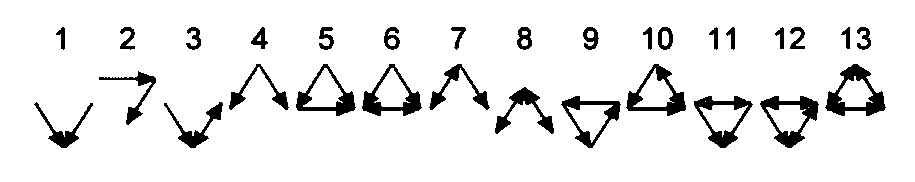
\includegraphics[width=0.8\textwidth]{triades} 
\caption{As 13 tríades e seus números de identificação. Adaptado de 
\cite{Milo2002}.} 
\label{fig:triades} 
\end{figure}

Analisamos as redes dos 65 sistemas em Java já mencionados e constatamos que em
todos eles a tríade de número 1 é a que aparece com maior frequência,
respondendo por 30\% a 90\% das tríades de cada rede. Já as redes metabólicas
\cite{Jeong2000} se diferenciam por apresentar predominância da tríade 2.

\renewcommand{\refname}{Referências Bibliográficas} \bibliographystyle{sbc}
\bibliography{rodrigo-mestrado,complex-networks,extra}

\end{document}

